%! Author = bedlamzd
%! Date = 15.03.2021

\documentclass[14pt]{extarticle}

% Preamble
%! Author = bedlamzd
%! Date = 16.02.2021

\usepackage{fontspec}
\usepackage{polyglossia}
\defaultfontfeatures{Ligatures=TeX}
\setdefaultlanguage{russian}
\setotherlanguage{english}
\setmainfont{PT Astra Serif}
\newfontfamily{\latinfont}{PT Astra Serif}
\newfontfamily{\cyrillicfont}{PT Astra Serif}
\newfontfamily{\cyrillicfonttt}{FreeMono}

\usepackage{geometry}

\usepackage{mathtools}
\usepackage{amsmath}
\usepackage{amssymb}
\usepackage{amsfonts}
\usepackage{graphicx}
\usepackage{float}
\usepackage{wrapfig}
\usepackage{subcaption}

\geometry{right=20mm}
\geometry{left=20mm}
\geometry{top=20mm}
\geometry{bottom=20mm}

\usepackage{indentfirst}
\usepackage[outputdir=out]{minted}

\usepackage{booktabs}
\usepackage{array}

\renewcommand{\theFancyVerbLine}{\ttfamily{\normalsize\oldstylenums{\arabic{FancyVerbLine}}}}
\renewcommand{\listingscaption}{Листинг}

\newminted{python}{autogobble, linenos, fontsize=\small}
\newmintinline{python}{fontsize=\small}
\newmintedfile{python}{autogobble, linenos, fontsize=\small, breakanywhere, breaklines}

\newminted{lua}{autogobble, linenos, fontsize=\small}
\newmintinline{lua}{fontsize=\small}
\newmintedfile{lua}{autogobble, linenos, fontsize=\small, breakanywhere, breaklines}

%\renewcommand{\thesubsection}{\arabic{subsection}}

\graphicspath{{../img/}}



% Document
\begin{document}

    \begin{titlepage}
    \begin{center}
        \begin{small}
            \textbf{Министерство науки и высшего образования Российской Федерации}

            \vspace{1em}

            ФЕДЕРАЛЬНОЕ ГОСУДАРСТВЕННОЕ АВТОНОМНОЕ ОБРАЗОВАТЕЛЬНОЕ\\
            УЧРЕЖДЕНИЕ ВЫСШЕГО ОБРАЗОВАНИЯ

            \vspace{1em}

            \textbf{<<НАЦИОНАЛЬНЫЙ ИССЛЕДОВАТЕЛЬСКИЙ УНИВЕРСИТЕТ ИТМО>>}
        \end{small}

        \vspace{13ex}

        Лабораторная работа №1\\
        по дисциплине <<Имитационное моделирование робототехнических систем>>
    \end{center}

    \vspace{14em}

    \begin{flushright}
        \noindent
        Выполнил:\\
        студент гр. R41341c\\
        Борисов М. В.

        \vspace{1em}
        Преподаватель:\\
        Бжихатлов И. А.
    \end{flushright}

    \vfill

    \begin{center}
        \large{Санкт-Петербург}\\
        2021 г.\\
    \end{center}
\end{titlepage}


    \section*{Цель работы}
    \begin{itemize}
        \item Средствами симулятора собрать модель схвата манипулятора
        \item Использовать сенсор для обнаружения объектов в схвате
        \item Написать скрипт активации схвата на основе данных датчика
    \end{itemize}

    \section*{Ход работы}

    Соберём из простейших элементов примитивный схват манипулятора. Для этого воспользуемся кубами и линейными
    актуаторами. Соответственно кубы представляют собой конкретные детали схвата, а актуаторы это некоторый виртуальный
    линейный мотор. При этом актуатору не обязательно находиться в непосредственном контакте с деталью, поскольку у него
    нет физических свойств.

    Добавив на левую часть схвата сенсор получим модель изображённую на рисунке~\ref{pic:wip gripper}.

    \begin{figure}[H]
        \centering
        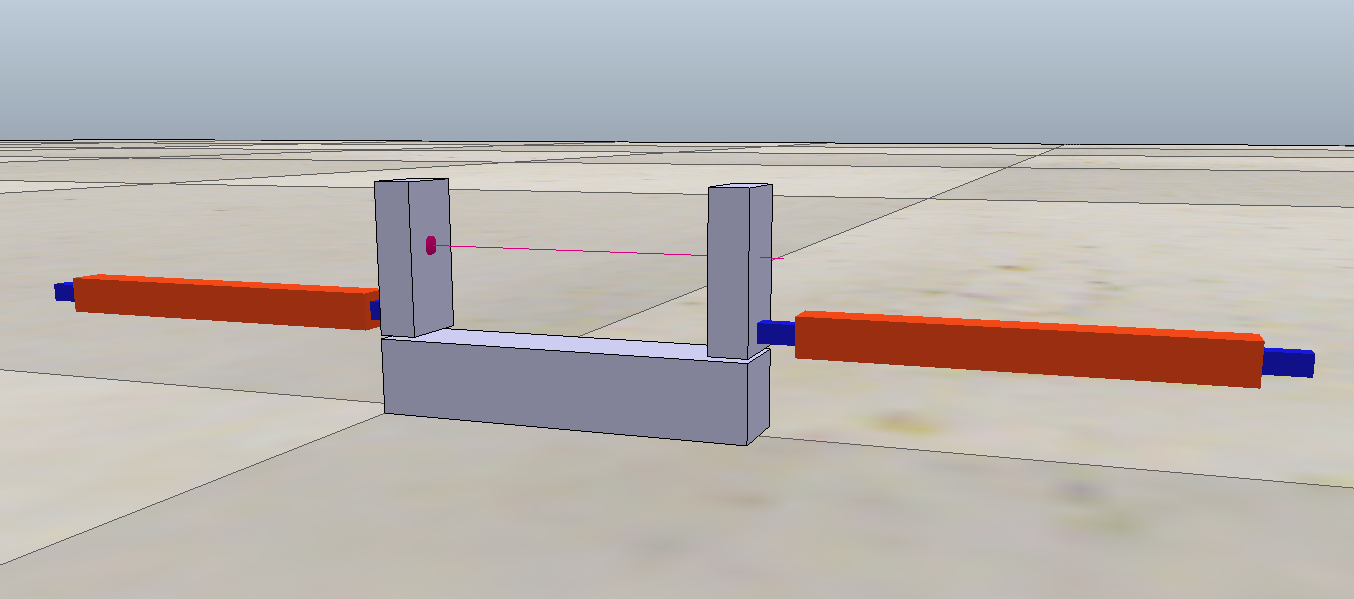
\includegraphics[width=0.75\textwidth]{gripper1.png}
        \caption{Модель схвата}
        \label{pic:wip gripper}
    \end{figure}

    \begin{figure}[H]
        \centering
        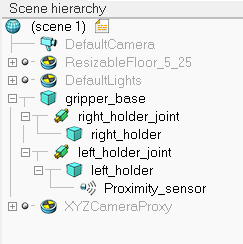
\includegraphics{tree.png}
        \caption{Дерево модели в процессе работы}
        \label{pic:wip tree}
    \end{figure}

    \begin{figure}[H]
        \centering
        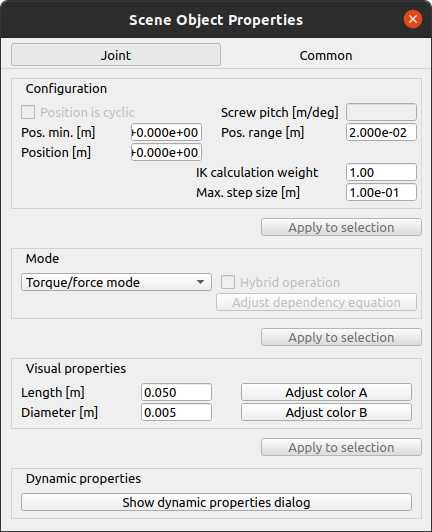
\includegraphics[width=0.4\textwidth]{joint_settings.png}
        \caption{Параметры линейного актуатора}
        \label{pic:joint settings}
    \end{figure}

    Добавим в сцену объект для обнаружения датчиком и напишем простой скрипт (Приложение~\ref{code:script}), который
    считывает с датчика данные и, как только в его пределах видимости появляется деталь, подаёт команду на схват.

    \begin{figure}[H]
        \centering
        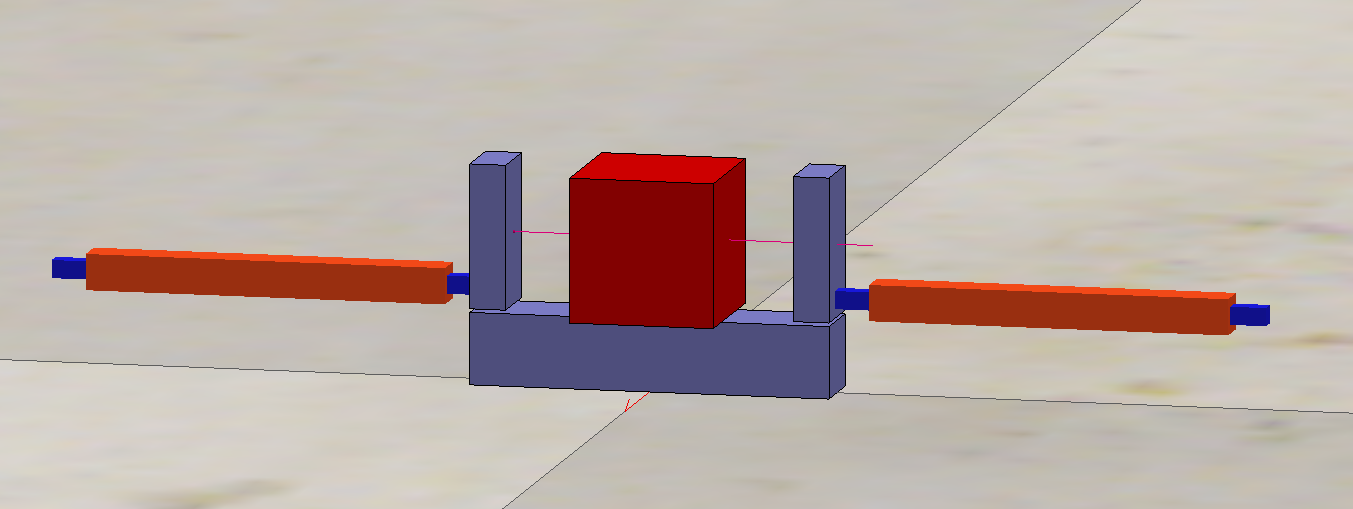
\includegraphics[width=0.75\textwidth]{final_scene.png}
        \caption{Схват с объектом для обнаружения}
        \label{pic:final scene}
    \end{figure}

    \begin{figure}[H]
        \centering
        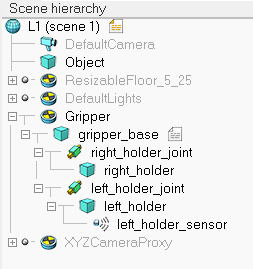
\includegraphics{final_tree.png}
        \caption{Дерево модели по окончанию работы}
        \label{pic:final tree}
    \end{figure}

    \section*{Вывод}
    В работе были изучены примитивы и простейший сенсор предоставляемые симулятором. Также в процессе
    были освоены базовые принципы языка программирования Lua, на котором пишутся скрипты для описания
    поведения объектов.


    \appendix
    \renewcommand{\thesection}{\Asbuk{section}}
    \section{Управляющий скрипт}\label{code:script}
    \luafile[frame=single]{../src/main.lua}


\end{document}
